%%%%%%%%%%%%%%%%%%%%%%%%%%%%%%%%%%%%%%%%%
% Programming/Coding Assignment
% LaTeX Template
%
% This template has been downloaded from:
% http://www.latextemplates.com
%
% Original author:
% Ted Pavlic (http://www.tedpavlic.com)
%
% Note:
% The \lipsum[#] commands throughout this template generate dummy text
% to fill the template out. These commands should all be removed when 
% writing assignment content.
%
% This template uses a Perl script as an example snippet of code, most other
% languages are also usable. Configure them in the "CODE INCLUSION 
% CONFIGURATION" section.
%
%%%%%%%%%%%%%%%%%%%%%%%%%%%%%%%%%%%%%%%%%

%----------------------------------------------------------------------------------------
%	PACKAGES AND OTHER DOCUMENT CONFIGURATIONS
%----------------------------------------------------------------------------------------

\documentclass{article}
\usepackage{amsmath}
\usepackage{fancyhdr} % Required for custom headers
\usepackage{lastpage} % Required to determine the last page for the footer
\usepackage{extramarks} % Required for headers and footers
\usepackage[usenames,dvipsnames]{color} % Required for custom colors
\usepackage{graphicx} % Required to insert images
\usepackage{listings} % Required for insertion of code
\usepackage{courier} % Required for the courier font
\usepackage{lipsum} % Used for inserting dummy 'Lorem ipsum' text into the template

% Margins
\topmargin=-0.45in
\evensidemargin=0in
\oddsidemargin=0in
\textwidth=6.5in
\textheight=9.0in
\headsep=0.25in

\linespread{1.1} % Line spacing

% Set up the header and footer
\pagestyle{fancy}
\lhead{\hmwkAuthorName} % Top left header
\chead{\hmwkClass\ (\hmwkClassInstructor\ \hmwkClassTime): \hmwkTitle} % Top center head
\rhead{\firstxmark} % Top right header
\lfoot{\lastxmark} % Bottom left footer
\cfoot{} % Bottom center footer
\rfoot{Page\ \thepage\ of\ \protect\pageref{LastPage}} % Bottom right footer
\renewcommand\headrulewidth{0.4pt} % Size of the header rule
\renewcommand\footrulewidth{0.4pt} % Size of the footer rule

\setlength\parindent{0pt} % Removes all indentation from paragraphs

%----------------------------------------------------------------------------------------
%	CODE INCLUSION CONFIGURATION
%----------------------------------------------------------------------------------------

\definecolor{MyDarkGreen}{rgb}{0.0,0.4,0.0} % This is the color used for comments
\lstloadlanguages{Perl} % Load Perl syntax for listings, for a list of other languages supported see: ftp://ftp.tex.ac.uk/tex-archive/macros/latex/contrib/listings/listings.pdf
\lstset{language=Perl, % Use Perl in this example
        frame=single, % Single frame around code
        basicstyle=\small\ttfamily, % Use small true type font
        keywordstyle=[1]\color{Blue}\bf, % Perl functions bold and blue
        keywordstyle=[2]\color{Purple}, % Perl function arguments purple
        keywordstyle=[3]\color{Blue}\underbar, % Custom functions underlined and blue
        identifierstyle=, % Nothing special about identifiers                                         
        commentstyle=\usefont{T1}{pcr}{m}{sl}\color{MyDarkGreen}\small, % Comments small dark green courier font
        stringstyle=\color{Purple}, % Strings are purple
        showstringspaces=false, % Don't put marks in string spaces
        tabsize=5, % 5 spaces per tab
        %
        % Put standard Perl functions not included in the default language here
        morekeywords={rand},
        %
        % Put Perl function parameters here
        morekeywords=[2]{on, off, interp},
        %
        % Put user defined functions here
        morekeywords=[3]{test},
       	%
        morecomment=[l][\color{Blue}]{...}, % Line continuation (...) like blue comment
        numbers=left, % Line numbers on left
        firstnumber=1, % Line numbers start with line 1
        numberstyle=\tiny\color{Blue}, % Line numbers are blue and small
        stepnumber=5 % Line numbers go in steps of 5
}

% Creates a new command to include a perl script, the first parameter is the filename of the script (without .pl), the second parameter is the caption
\newcommand{\perlscript}[2]{
\begin{itemize}
\item[]\lstinputlisting[caption=#2,label=#1]{#1.pl}
\end{itemize}
}

%----------------------------------------------------------------------------------------
%	DOCUMENT STRUCTURE COMMANDS
%	Skip this unless you know what you're doing
%----------------------------------------------------------------------------------------

% Header and footer for when a page split occurs within a problem environment
\newcommand{\enterProblemHeader}[1]{
\nobreak\extramarks{#1}{#1 continued on next page\ldots}\nobreak
\nobreak\extramarks{#1 (continued)}{#1 continued on next page\ldots}\nobreak
}

% Header and footer for when a page split occurs between problem environments
\newcommand{\exitProblemHeader}[1]{
\nobreak\extramarks{#1 (continued)}{#1 continued on next page\ldots}\nobreak
\nobreak\extramarks{#1}{}\nobreak
}

\setcounter{secnumdepth}{0} % Removes default section numbers
\newcounter{homeworkProblemCounter} % Creates a counter to keep track of the number of problems

\newcommand{\homeworkProblemName}{}
\newenvironment{homeworkProblem}[1][Problem \arabic{homeworkProblemCounter}]{ % Makes a new environment called homeworkProblem which takes 1 argument (custom name) but the default is "Problem #"
\stepcounter{homeworkProblemCounter} % Increase counter for number of problems
\renewcommand{\homeworkProblemName}{#1} % Assign \homeworkProblemName the name of the problem
\section{\homeworkProblemName} % Make a section in the document with the custom problem count
\enterProblemHeader{\homeworkProblemName} % Header and footer within the environment
}{
\exitProblemHeader{\homeworkProblemName} % Header and footer after the environment
}

\newcommand{\problemAnswer}[1]{ % Defines the problem answer command with the content as the only argument
\noindent\framebox[\columnwidth][c]{\begin{minipage}{0.98\columnwidth}#1\end{minipage}} % Makes the box around the problem answer and puts the content inside
}

\newcommand{\homeworkSectionName}{}
\newenvironment{homeworkSection}[1]{ % New environment for sections within homework problems, takes 1 argument - the name of the section
\renewcommand{\homeworkSectionName}{#1} % Assign \homeworkSectionName to the name of the section from the environment argument
\subsection{\homeworkSectionName} % Make a subsection with the custom name of the subsection
\enterProblemHeader{\homeworkProblemName\ [\homeworkSectionName]} % Header and footer within the environment
}{
\enterProblemHeader{\homeworkProblemName} % Header and footer after the environment
}

%----------------------------------------------------------------------------------------
%	NAME AND CLASS SECTION
%----------------------------------------------------------------------------------------

\newcommand{\hmwkTitle}{FE-Assignment\ \#04} % Assignment title
\newcommand{\hmwkDueDate}{Monday,\ February\ 15,\ 2016} % Due date
\newcommand{\hmwkClass}{MA\ 374} % Course/class
\newcommand{\hmwkClassTime}{} % Class/lecture time
\newcommand{\hmwkClassInstructor}{} % Teacher/lecturer
\newcommand{\hmwkAuthorName}{Silvi Pandey(130123045)} % Your name

%----------------------------------------------------------------------------------------
%	TITLE PAGE
%----------------------------------------------------------------------------------------

\title{
\vspace{2in}
\textmd{\textbf{\hmwkClass:\ \hmwkTitle}}\\
\normalsize\vspace{0.1in}\small{Due\ on\ \hmwkDueDate}\\
\vspace{0.1in}\large{\textit{\hmwkClassInstructor\ \hmwkClassTime}}
\vspace{3in}
}

\author{\textbf{\hmwkAuthorName}}
\date{} % Insert date here if you want it to appear below your name

%----------------------------------------------------------------------------------------

\begin{document}

\maketitle

%----------------------------------------------------------------------------------------
%	TABLE OF CONTENTS
%----------------------------------------------------------------------------------------

%\setcounter{tocdepth}{1} % Uncomment this line if you don't want subsections listed in the ToC


\newpage

%----------------------------------------------------------------------------------------
%	PROBLEM 1
%----------------------------------------------------------------------------------------

% To have just one problem per page, simply put a \clearpage after each problem


\begin{center}
\textbf{PROBLEM - 1}
\end{center}

Consider three assets with the following mean return vector and covariance matrix:
$$M = [0.1 , 0.2 , 0.15]$$

\[C =
\begin{bmatrix}
     0.005 & -0.010 & 0.004\\
	 -0.010 & 0.040 & -0.002\\
	  0.004 & -0.002 & 0.023
\end{bmatrix}
\]


(a) Construct and plot the Markowitz efficient frontier using the above data.\\
(b) Tabulate the weights, return and risk of the portfolios for 10 different values on the efficient frontier.\\
(c) For a 15 \% risk, what is the maximum and minimum return and the corresponding portfolios ?\\
(d) For a 18 \% return, what is the minimum risk portfolio ?\\
(e) Assuming the risk free return rf = 10\%, compute the market portfolio. Also determine and plot the
Capital Market Line.\\
(f) Find two portfolios (consisting of both risky and risk free assets) with the risk at 10\% and 25\%.

\begin{center}
\textbf{SOLUTION}
\end{center}

\textbf{Part a}

\begin{center}
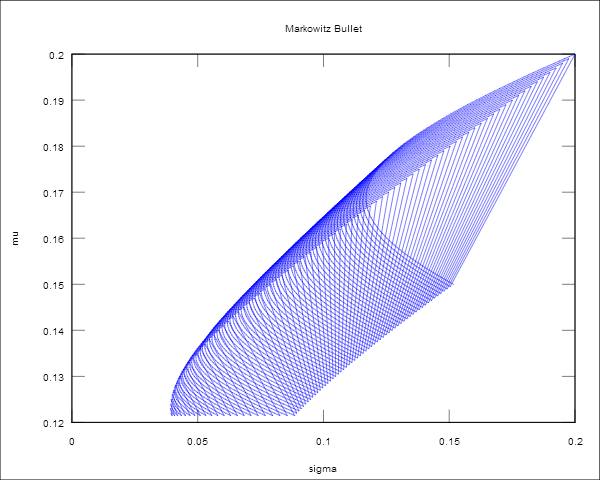
\includegraphics[width=80mm]{Markowitz_Bullet}
\end{center}
The above figure gives the feasible set of the portfolio weights i.e when $w_{1} + w_{2} + w_{3} = 1$ where $w_{i}$ is the weight of the $i_{th}$ stock in the portfolio.
\begin{center}
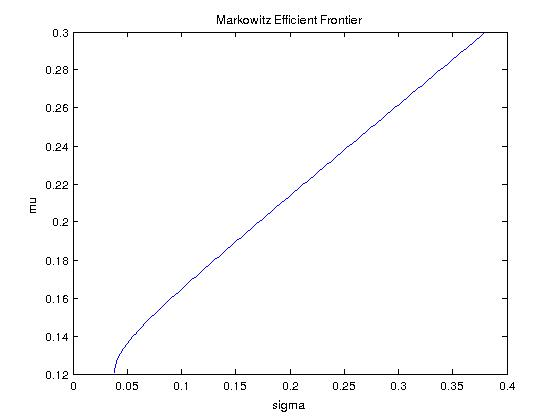
\includegraphics[width=80mm]{Markowitz_Efficient_Frontier}\\
Markowitz Efficient Frontier
\end{center}
Derivation of Markowitz Efficient Frontier :\\
Markowitz Efficient Frontier is the pair of ($\sigma$ , $\mu$) values such the the risk $\sigma$ involved with a given value of $\mu$ is minimum.\\\\
To minimize :
$$w C w^{'}$$
Subject to :
$$w m^{'} = \mu \quad wu^{'} = 1$$
where w : weight vector of the risky assets in the portfolio , C : Covariance matrix , m : vector of the expected return of the assets and u : row vector with n 1's where n is the number of assets.
$$G(w,\lambda_{1},\lambda_{2}) = wCw' - \lambda_{1}(wm' - \mu) - \lambda_{2}(wu' - 1)$$
To minimize the variance : $\frac{dG}{dw} = 0$ , $\frac{dG}{d\lambda_{1}} = 0$ , $\frac{dG}{d\lambda_{2}} = 0$
$$w = \frac{\lambda_{1}}{2}mC^{-1} + \frac{\lambda_{2}}{2}uC^{-1}$$
After all the calculations the weight vector obtained is of the form :
$$w = \mu a + b$$
where a and b are n dimentional vectors.\\\\
\textbf{Part b}\\
The following are the weight vectors, expected rate of returns and the risk for 10 different portfolios on the efficient frontier.
\begin{center}
\begin{tabular}{ |c|c|c|c| } 
 \hline
 No. & Weight Vector & Return & Risk\\
 \hline
1 & [0.818704 , 0.238720 , -0.057424] & 0.121001 & 0.038427\\
2 & [0.804392 , 0.244408 , -0.048800] & 0.122001 & 0.038485\\
3 & [0.790080 , 0.250096 , -0.040176] & 0.123001 & 0.038659\\
4 & [0.775768 , 0.255784 , -0.031553] & 0.124001 & 0.038947\\
5 & [0.761456 , 0.261473 , -0.022929] & 0.125001 & 0.039347\\
6 & [0.747144 , 0.267161 , -0.014305] & 0.126001 & 0.039855\\
7 & [0.732832 , 0.272849 , -0.005681] & 0.127001 & 0.040468\\
8 & [0.718520 , 0.278537 ,  0.002943] & 0.128001 & 0.041180\\
9 & [0.704208 , 0.284225 ,  0.011567] & 0.129001 & 0.041987\\
10 & [0.689897 , 0.289913 , 0.020191] & 0.130001 & 0.042883\\
 \hline
\end{tabular}
\end{center}
\textbf{Part c}\\\\
\begin{center}
\includegraphics[width=80mm]{Part3}\\
Maximum-Minimum return for 15\% Risk
\end{center}
\newpage
\textbf{Part d}\\\\
\begin{center}
\includegraphics[width=80mm]{Part4}\\
Minimum Risk for 18\% Return
\end{center}

\textbf{Part e}\\
Derivation of Market Portfolio :\\  
To maximize :
$$\frac{wm' - R}{\sqrt{wCw'}}$$
Subject to :
$$wu' = 1$$
where w : weight vector of the risky assets in the portfolio , C : Covariance matrix , m : vector of the expected return of the assets , R : risk free return and u : row vector with n 1's where n is the number of assets.
$$G(w,\lambda_{1},\lambda_{2}) = wCw' - \lambda(wu' - 1)$$
To maximize the slope : $\frac{dG}{dw} = 0$ , $\frac{dG}{d\lambda} = 0$
$$w = \frac{(m-Ru)C^{-1}}{(m-Ru)C^{-1}u'}$$
A portfolio with weight given by the above expression is called the market portfolio. \\\\
Derivation of Capital Market Line :\\
Capital Market line is the line joining $(0,R)$ and $(\sigma_{m},\mu_{m})$ given by :
$$\mu = R + \frac{(\mu_{m}-R)}{\sigma_{m}}\sigma$$
\begin{center}
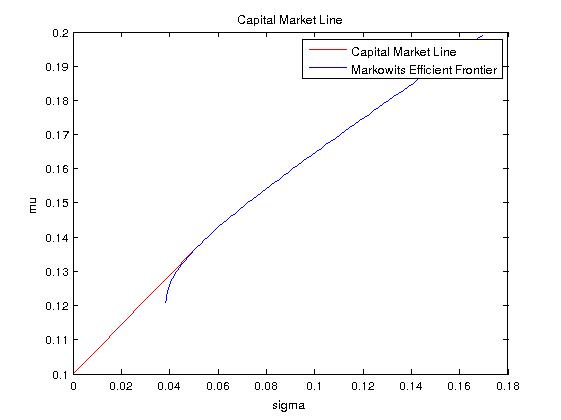
\includegraphics[width=80mm]{Capital_Market_line}
\end{center}
The market portfolio is :\\
weight vector : [0.593750 , 0.328125 , 0.078125]\\
Mean return : 0.13672\\
Standard Deviation : 0.050811\\\\
\textbf{Part f}\\
- Market Portfolio : Risk : $\sigma_{m}$ , Mean Return : $\mu_{m}$ , Weight : $w_{1}$\\
- Risk Free Assets : Risk : $\sigma_{2}$ , Mean Return : $\mu_{2}$ , Weight : $w_{2}$\\
Risk associated with Risk Free Assets will be zero, hence $\sigma_{2} = 0$.\\
$w_{1} + w_{2} = 1$

$$\sigma^{2} = w_{1}^{2}\sigma_{m}^{2} + w_{2}^{2}\sigma_{2}^{2} + 2w_{1}w_{2}\rho\sigma_{m}\sigma_{2}$$
$$\sigma^{2} = w_{1}^{2}\sigma_{m}^{2}$$
$$w_{1} = \frac{\sigma}{\sigma_{m}}$$
When $\sigma = 0.10, w_{2} = 1.403, w_{1} = -0.403$\\
When $\sigma = 0.15, w_{2} = 1.718, w_{1} = -0.718$\\

\begin{center}
\textbf{PROBLEM - 2}
\end{center}
Obtain data (from online resources) for 10 stocks each with 50 data points all taken at the same dates (preferably spread over a year at equal intervals). Put this data and it’s details in a single Excel/CSV file. Using the data and
assuming 7\% risk free return:\\
(a) Construct and plot the Markowitz efficient frontier.\\
(b) Determine the market portfolio.\\
(c) Determine and plot the Capital Market Line.\\
(d) Determine and plot the Security Market Line for all the 10 assets.\\
\begin{center}
\textbf{SOLUTION}
\end{center}
The stocks chosen are that of :\\
ADITYA\_BIRLA , ALPHABET (GOOGLE) , AMAZON , FACEBOOK , HYATT , MTNL , ORACLE , TAJ , TATA\_MOTOR , YAHOO\\
The data has been taken from 'Yahoo Finance' and the dates are from 1st January 2015 to 1st January 2016 (taken weekly).The expected return and variance have been calculated by taking the mean of all the returns obtained in every weekly interval.It has been assumed that the returns are independent i.e the covariance is 0 for two different stocks.  \\

\textbf{Part a}\\
\begin{center}
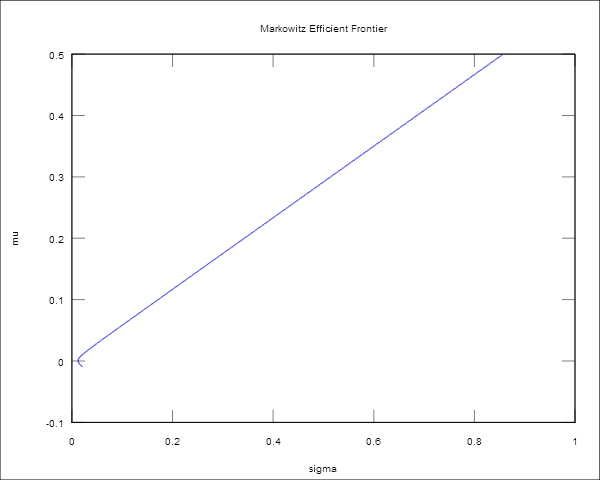
\includegraphics[width = 70mm]{onlineMarkowitzEfficientFrontier}\\
Markowitz Efficient Frontier
\end{center}
\newpage
\textbf{Part b}\\
The market portfolio : \\
\begin{center}
\includegraphics[width = 100 mm]{Capture}
\end{center}

\textbf{Part c}\\
\begin{center}
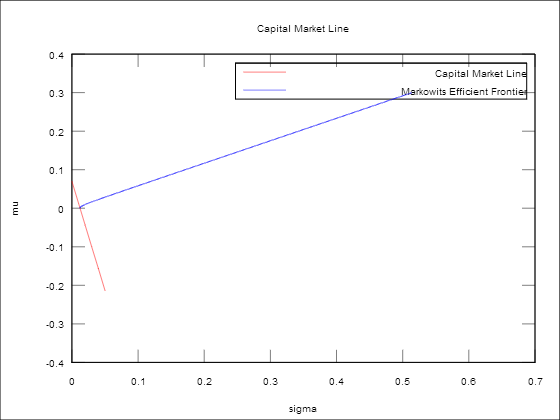
\includegraphics[width = 80mm]{onlineCapitalMarketLine}\\
Capital Market Line
\end{center}
\end{document}
